\chapter{QHS Compiler} \label{cha:4-QHS_Compiler}
Die QHS Sprache besteht natürlich aus Wörtern. Im Kontext von QHS werden diese Wörter im folgenden als Orders benannt. Diese Orders weisen 3 verschiedenen Typen auf. Identifiers, Instructions und LiteralCode.
Bei Identifiers handelt es sich um die in Kapitel \ref{cha:3-Meine_Idee} bereits erwähnten Macros. Instructions sind einfache vorprogrammierte Anweisungen an den QHScompiler und LiteralCode ist Text, der exakt so wie er steht,
in den Output-File geschrieben wird. Wie diese 3 Orders genau funktionieren wird in Abschnitt \ref{sec:qhs-execute} ausführlicher erklärt.

Der Compilation von QHS steht ein einfacher Zyklus zugrunde, dessen Vorbild der Von-Neumann Zyklus ist.

\begin{figure}[h!]
    \centering
    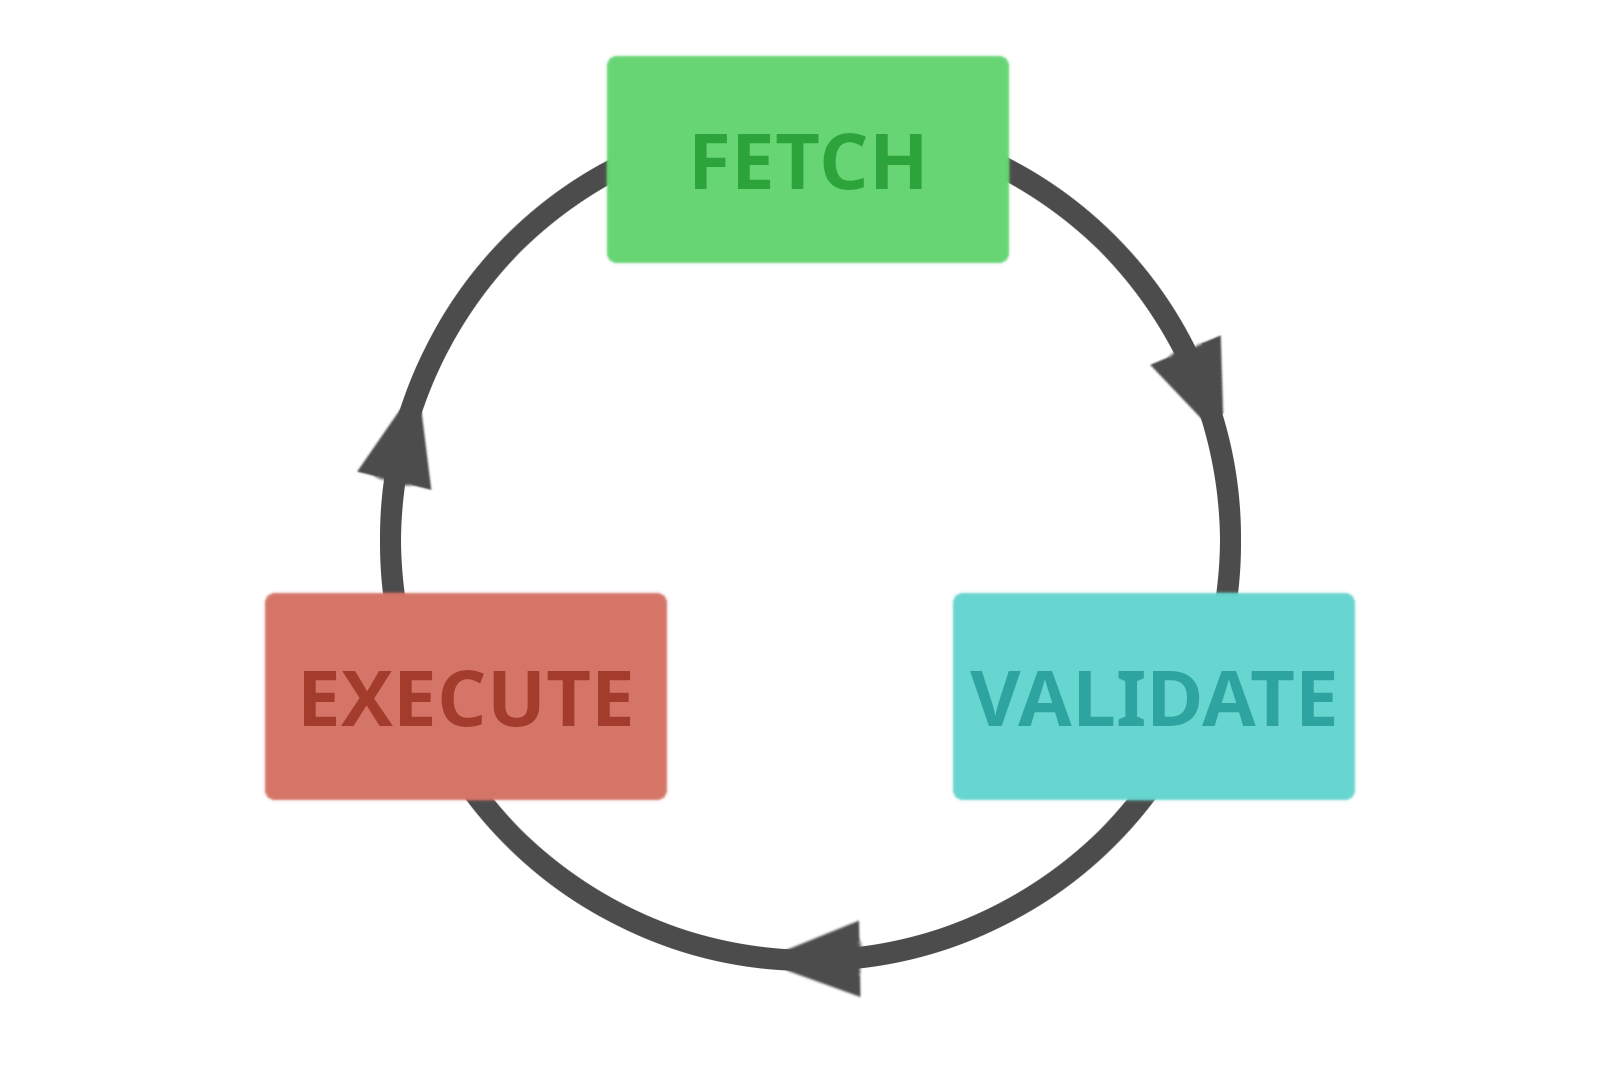
\includegraphics[scale=0.6]{resources/qhs-cycle.png}
    \caption{Zyklus der QHS Compilation}
    \label{fig:qhs-cycle}
\end{figure}

\section{Fetch} \label{sec:qhs-fetch}
Der QHS-Zyklus beginnt mit dem ersten Fetch. Dabei wird die erste Order aus dem Inputfile extrahiert. Eine Order weist einen der drei Typen Identifier, Instruction oder Literal-Code auf. Diese sind mit folgenden RegEx definiert.
Whitespaces dienen als Trennung zwischen zwei Orders und werden ignoriert.

\begin{table}[h]
    \centering
    \begin{tabular}{ll}
    \multicolumn{1}{l|}{identifier}        & \textless{}identiferChar\textgreater{}*                           \\ \hline
    \multicolumn{1}{l|}{instruction}       & \# \textless{}identiferChar\textgreater{}*                        \\ \hline
    \multicolumn{1}{l|}{literalCode}       & ".*"                                                              \\
                                           &                                                                   \\
    \textless{}identiferChar\textgreater{} & = {[}\textasciicircum{}\# "\textless{}whitespace\textgreater{}{]} \\
    \textless{}whitespace\textgreater{}    & = SPACE | NEWLINE | TAB
    
    \end{tabular}
\end{table}

Auffällig gegenüber einem traditionellen Compiler ist hierbei, dass kaum zwischen Zeichen differenziert wird. Während die Lexical Analysis traditionell zwischen vielen verschiedenen Tokens unterscheidet,
sind für den QHScompiler alle Zeichen bis auf \# und " gleich.

Es ist hierbei möglich bestimmte Orders voran zu stellen, die anstelle der nächsten Order im Inputfile gefetched werden. Dies geschieht mit Hilfe des Fetch-Stacks auf den eine Liste an Orders gepushed werden kann.
Auf diesen Fetch-Stack kann während jeder der drei Schritte des Zyklus, meist jedoch während Execute, gepushed werden. Wie der Name Stack schon sagt, funktioniert der Fetch-Stack mit Last-In First-Out.
Die Hauptanwendung des Fetch-Stacks wird im Abschnitt \ref{sec:qhs-execute} ausgeführt.

\begin{figure}[h!]
    \centering
    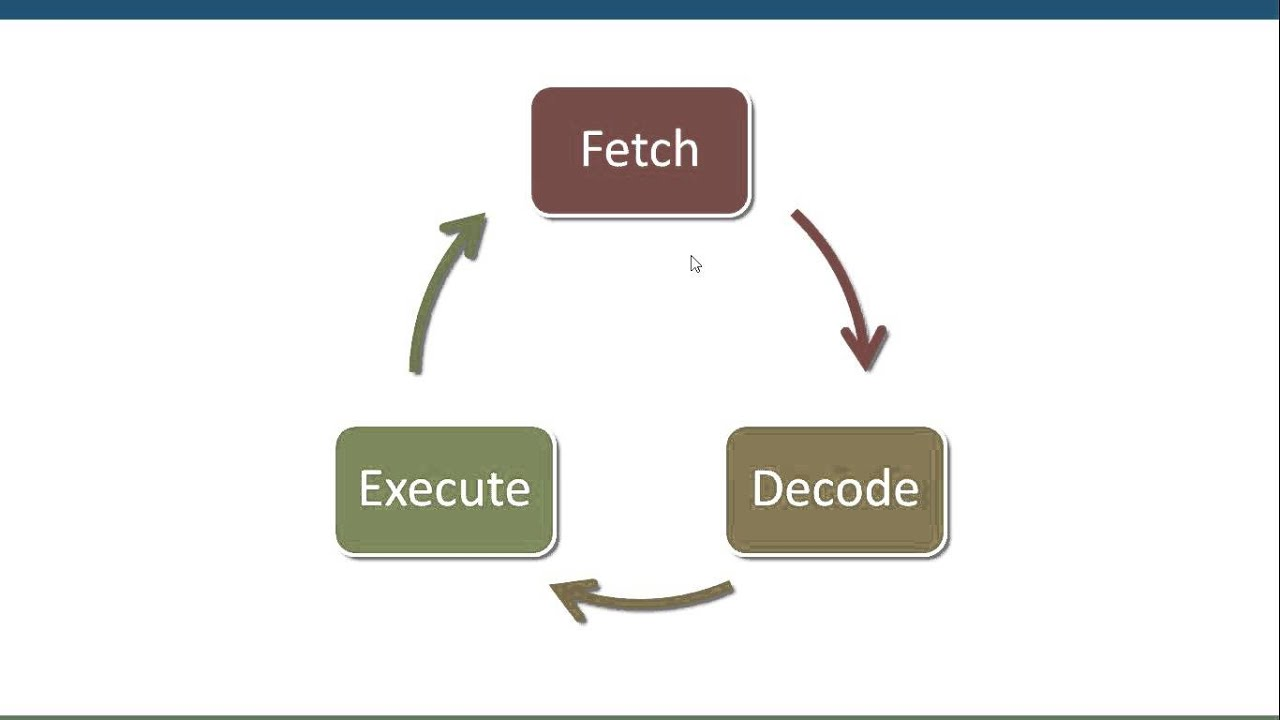
\includegraphics[scale=0.3]{resources/TEMP_von-neumann-cycle.jpg}
    \caption{TEMP! Struktur des Fetch-Stacks}
    \label{fig:fetch-stack}
\end{figure}

Wenn eine Liste an Orders komplett gefetched wurde, wird diese vom Stack gelöscht. Der Inputfile befindet sich auf dem letzten Platz des Fetch-Stacks und wird somit nur verwendet, wenn der Stack ansonsten komplett leer ist.
Die Compilation wird beendet, sobald keine Order mehr auf dem Fetch-Stack übrig ist.

\section{Validate} \label{sec:qhs-Validate}
Nachdem eine Order gefetched wurde, wird diese an Validate weitergegeben. Während dem Validate Schritt kommt die OrderQueue ins Spiel. Hierbei handelt es sich um eine Liste an Orders, der Form First-In First-Out.
Die Anwendung Aufgabe der OrderQueue ist das Speichern und spätere Ausführen von Orders. Die OrderQueue kann mit Hilfe von Instructions, die im Abschnitt \ref{sec:qhs-execute} weiter ausgeführt werden, aktiviert und deaktiviert werden.
Wenn nun eine Order in den Validate Schritt gelangt und die OrderQueue aktiviert ist, wird diese Order der OrderQueue hinzugefügt. Der Execute Schritt wird danach übersprungen und der Zyklus beginnt von neuem bei Fetch.
Die Order wurde ohne ausgeführt zu werden auf der OrderQueue gespeichert. Später ist es nun möglich diese Order mit Hilfe von Instructions, die im Abschnitt \ref{sec:qhs-execute} weiter thematisiert werden, 
von der OrderQueue zu entfernen und auszuführen. Bestimmte Instructions und Identifiers können jedoch OrderQueue-Proof, also immun gegen die OrderQueue, gemacht werden. Diese werden, auch wenn die OrderQueue aktiv ist, 
normal an Execute weitergegeben. Dies ist zum Beispiel besonders bei der Instruction, die die OrderQueue wieder deaktiviert, wichtig. Da diese Instruction sonst nicht ausgeführt und somit die OrderQueue nie mehr deaktiviert wird.
LiteralCode kann nicht Code-Queue-Proof sein.

MAYBE CODESTACK FIGURE

Ist die OrderQueue deaktiviert oder die Order OrderQueue-Proof, wird diese an den letzten Schritt Execute weitergegeben.

\section{Execute} \label{sec:qhs-execute}
Execute ist der letzte Schritt des Zyklus. Und hier wird nun auch endlich der tatsächliche Assembly Code generiert. Je nach Typ der Order, Identifier, Instruction oder Literal-Code, läuft Execute sehr unterschiedlich ab.

\subsection{Identifier}
Ein Identifier ist eine Zusammenfassung von mehreren Orders. Diese sind in einem Environment definiert. Hierbei handelt es sich um eine einfach Map (Dictionary), \textbf{die einen Identifier als string mit einer Liste an Orders verknüpft}.
Wenn nun ein Identifier in den Execute Schritt kommt, werden die dazugehörige Liste an Orders auf den Fetch-Stack aus Abschnitt \ref{sec:qhs-fetch} gepushed.
Beim nächsten Fetch werden nun die zum Identifier gehörenden Orders zurückgegeben. Um Grunde wird der Identifier mit seinen Orders ersetzt.

Environments sind hierbei in einer Linked-List gespeichert. Somit können neue Environments zu dieser Liste hinzugefügt und von der Liste entfernt werden. Das unterste Element der Liste ist hierbei das älteste und das oberste Element das neuste.
Bei der Definition eines Identifiers wird dieser immer zum obersten Environment hinzugefügt. Definitionen des gleichen Identifiers in älteren Environments werden nicht überschrieben oder gelöscht.
Bei der Abfrage nach einem Identifier wird immer die neuste vorhandene Definition zurückgegeben. Ist keine vorhanden, wird ein Error ausgegeben.

\subsection{Literal-Code}
Literal-Code ist der Weg wie der QHS-Compiler Assembly Code generiert. Dieser ist sehr simpel. Wenn Literal-Code in den Execute Schritt gelangt, wird alles was zwischen den " Zeichen steht in das Output-Dokument geschrieben.

\subsection{Instructions}
Instructions sind die komplexeste Order für den Execute Schritt. Für jede Instruction ist im QHS-Compiler eine Funktion definiert, die ausgeführt wird, wenn diese Instruction in den Execute Schritt gelangt.
Diese Funktionen können Variabeln im QHS-Compiler speichern, den OrderQueue aktivieren, Identifier definieren und noch viel mehr. Folgend sind ein paar der wichtigsten Instructions aufgelistet.

\begin{table}[H]
    \centering
    \begin{tabularx}{\textwidth}{l|X}
    \textbf{\#enterOrderQueue}      & Aktiviert die OrderQueue. \\ \hline
    \textbf{\#exitOrderQueue}       & Deaktiviert die OrderQueue. \\ \hline
    \textbf{\#assign}               & Das erste Element der OrderQueue muss ein Identifier sein. Der Rest der Orders auf OrderQueue wird als Definition für diesen Identifier festgelegt. \\ \hline
    \textbf{\#assignToOne}          & Wie \#assign, jedoch wird nach dem Identifier nur eine weitere Order von der OrderQueue genommen und als Definition für den Identifier verwendet. \\ \hline
    \textbf{\#force}                & Die nächste Order wird nach Fetch sofort an Execute weitergegeben. Überspringt Validate und somit die OrderQueue. \\ \hline
    \textbf{\#orderEnqueue}         & Die nächste Order wird sofort der OrderQueue hinzugefügt, auch wenn diese Order OrderQueue-Proof wäre. Execute wird übersprungen. \\ \hline
    \textbf{\#orderFrontEnqueue}    & Ähnlich wie \#orderEnqueue. Die Order wird jedoch auf den obersten Platz der OrderQueue gesetzt. \\ \hline
    \textbf{\#deepFetch}            & Wird mit der ersten Order der zweitobersten Liste an Order auf dem Fetch-Stack. Ermöglicht den Zugriff auf den Inputfile innerhalb einer Identifier-Definition. \\ \hline
    \textbf{\#pushEnv}              & Ein neues Environment wird der Environment Linked-List hinzugefügt. \\ \hline
    \textbf{\#popEnv}               & Das neuste Environment der Environment Linked-List wird gelöscht.
        
    \end{tabularx}
\end{table}

ADD put in front and addIdentifier and lightForce

Der QHScompiler umfässt \textbf{33} Instructions, wobei \textbf{5} dieser nur für Debugging des Compilers dienen.

\section{Bringing it all together}
Und das war's. Dies ist der gesamte QHScompiler. Im Vergleich zu einem traditionellen Compiler wirkt der QHScompiler fast schon \textbf{armselig}. Und dies hat einen einfachen Grund. Der QHScompiler ist zwar \textbf{vollendet},
die dazugehörige Sprache QHS jedoch noch lange nicht. Es ist zwar grundsätzlich durch LiteralCode möglich jedes Programm QHS zu schreiben, jedoch handelt es sich dann dabei einfach nur um Assembly Code.
Doch der Aufbau des QHScompilers ermöglicht es mithilfe von Identifiern eine komplexere Programmiersprache zu definieren.

\subsection{Shortcuts}
Um die Leserlichkeit von QHS zu verbessern, werden ein paar Identifiers anstelle der umständlichen Instruction Namen definiert.

\begin{table}[H]
    \centering
    \begin{tabular}{l|l}
    \textbf{{[}}                 & \#enterOrderStack              \\ \hline
    \textbf{{]}}                 & \#exitOrderStack               \\ \hline
    \textgreater{}\textgreater{} & \#assign                       \\ \hline
    \textbf{-\textgreater{}}     & \#assignToOne                  \\ \hline
    \textbf{!}                   & \#force                        \\ \hline
    \textbf{?!}                  & \#lightForce                   \\ \hline
    \textbf{\textbackslash{}n}   & Eine neue Zeile im Output-File
    \end{tabular}
\end{table}

Weiter wird in den Kommentaren innerhalb der Beispiele Pseudo-Code verwendet, um den QHS Code besser zu erklären. Kommentare können über mehrere Zeilen reichen und beginnen immer mit /* und enden mit */.
Der Kommentar /* X = "hello" \#pushEnv */ würde bedeuten, dass der Identifier X zu den Orders "hello" (LiteralCode) und \#pushEnv (Instruction) definiert wurde. 

\subsection{Identifier Parameters and Return}
Parameter and Return through OrderQueue or PutInFront
lateArg>> ?

\subsection{Variablen} \label{sec:qhs-vars}
Die Umsetzung von Variablen in QHS ist simpel. Zuerst soll die Grösse der Variabel vom Stack abgezogen werden. Dann wird ein für den Identifier ein Variabelnamen definiert, der zu der Position der Variabel auf dem Stack zeigt.
Mit nur LiteralCode in QHS lässt sich dies wie folgt ausdrücken:

\begin{lstlisting}[language=QHS, caption=Beispiel einer Variabel in QHS]
"sub rsp, 4" \n
[ a "[rbp-4]" ] >> /* a = "[rbp-4]" */

"add " a ", 5"

%\noindent\hrulefill Output\noindent\hrulefill%
sub rsp, 4
add [rbp-4], 5
\end{lstlisting}

Jedoch ist dies noch nicht besonders angenehm. Weiter lässt sich zum Beispiel ein Var Identifier definieren, der die Grösse der Variabel als Argument annimmt OrderQueue. Um die in vielen Programmiersprachen geläufige Syntax
einer Variabel Definition beizubehalten, wird der Variabel Name mithilfe der \#deepFetch Instruction beschafft.

\begin{lstlisting}[language=QHS, caption=Definition einer Variable mit var Identifier]
[ var ]
[
    #putInFront size ->             /* size = argument1 */
    [ name ?! #deepFetch ] >>       /* name = Was nach dem var Identifier folgt */

    "sub rsp, " size \n

    [ ?! name "[rbp-4]" ] >>        /* var = "[rbp-4]" */
] >> 

[ "4" ] var a 

"add " a ", 5"
    
%\noindent\hrulefill Output\noindent\hrulefill%
sub 4
add [rbp-4], 5
\end{lstlisting}

Ganz so richtig funktioniert dies aber noch nicht. Momentan erhält jede Variable die Addresse rbp-4 und somit überschreiben sich die Variablen gegenseitig. Der momentane rbp-Offset muss also gespeichert und erhöht werden.
Hierzu wird bereits am Anfang des Programms ein Identifier rbpOffset als 0 definiert. Mithilfe der \#addToIdentifier Instruction, lässt sich daraufhin rbpOffset erhöhen. Dies kann wiefolgt aussehen.

\begin{lstlisting}[language=QHS, caption=Definition einer Variable mit rbpOffset]
[ rbpOffset "0" ] >>    /* rbpOffset = "0" */

[ var ]
[
    #putInFront size ->             /* size = argument1 */
    [ name ?! #deepFetch ] >>       /* name = Was nach dem var Identifier folgt */

    "sub rsp, " size \n

    [ rbpOffset ?! size ] #addToIdentifier  /* rbpOffset += size */

    [ ?! name "[rbp-" ?! rbpOffset "]" ] >> /* var = "[rbp-OFFSET]" */
] >> 

[ "4" ] var a 
[ "8" ] var b 

"add " a ", 5"
"sub " b ", 10"
    
%\noindent\hrulefill Output\noindent\hrulefill%
sub rsp, 4
sub rsp, 8
add [rbp-4], 5
sub [rbp-12], 10
\end{lstlisting}

Zuletzt lässt sich das umständliche Hinzufügen der Grösse der Variable sowie der Var Identifier unter einem Identifier zusammenfassen. Dies wäre passenderweise die bekannte Bezeichnung für den Variabel Typen.

\begin{lstlisting}[language=QHS, caption=Definition einer Variable mit int Identifier]
(...)

[ int ] 
[
    [ "4" ] var
] >>
    
int a 
int var b 
    
"add " a ", 5"
"sub " b ", 10"
        
%\noindent\hrulefill Output\noindent\hrulefill%
sub rsp, 4
sub rsp, 8
add [rbp-4], 5
sub [rbp-12], 10
\end{lstlisting}

So sieht eine Variabel Definition genau so aus, wie es in anderen Programmiersprachen gebräuchlich ist. Der Shortcut ; ist hierbei optional.

\subsection{Funktionen}
Funktionen sind im Vergleich zu Variablen deutlich komplizierter. \textbf{Daher soll hierbei nur auf zwei der Problematiken an Funktionen behandelt werden.}

Zum Schluss sollte eine Funktionsdefinition wie folgt aussehen:


\begin{lstlisting}[language=QHS, label=eg:qhs-function_goal, caption=Ziel für die Definition einer Funktion in QHS]
int foo ( int param1 , int param2 )
{
    (...)
}
            
%\noindent\hrulefill Output\noindent\hrulefill%
foo:
(...)
\end{lstlisting}

Hier lässt sich bereits ein erstes Problem feststellen. Im vorherigen Abschnitt \ref{sec:qhs-vars} wurde der Int Identifier für eine Variabel Definition verwendet. 
Das int aus Beispiel \ref{eg:qhs-function_goal} würde vom QHScompiler also als eine Variabel Definition verstanden werden. Der Unterschied zwischen Funktions und Variabel Definition besteht hierbei in den Klammern,
die auf den \textbf{Namen} folgen. Der QHScompiler müsste also beim Int Identifier nach vorne schauen, ob sich eine Klammer nach dem \textbf{Namen} befindet, und folglich eine Variabel oder Funktionsdefinition ausführen.
Dies ist jedoch aufgrund des einfachen Designs des QHScompilers nicht möglich. Er kann bloss Orders ausführen, nicht jedoch überprüfen, ob eine Order vorhanden ist. Glücklicherweise lässt sich dieses Problem jedoch lösen,
ohne eine Änderung am QHScompiler vorzunehmen. Die Lösung basiert darauf beim Int Identifier sowohl eine Variabel als auch eine Funktionsdefinition vorzubereiten, aber keine der beiden bereits auszuführen.
Weiter wird nun eine Klammer als Identifier für eine Funktionsdefinition definiert. Sowie ein Semikolon als Variabeldefinition. Befindet sich nach dem \textbf{Namen} also eine Klammer, wird eine Funktionsdefinition ausgeführt.
Ist dort aber ein Semikolon wird eine Variabeldefinition durchgeführt. Dieses Konzept wird weiterführend als DelayedExecute beschrieben. Das ganze könnte dann wie folgt aussehen:

\begin{lstlisting}[language=QHS, caption=Implementation eines DelayedExecute für Definitionen]
[ function ]
[
    #putInFront returnSize ->   /* size = argument1 */
    #putInFront name ->         /* name = argument2 */

    [ ?! name ] #orderToLiteral ":" \n      /* "foo:" */
] >>

[ definition ]
[
    #putInFront size ->             /* size = argument1 */
    [ name ?! #deepFetch ] >>       /* name = Was nach dem var Identifier folgt */

    [ ; ]
    [
        [ #orderEnqueue ! size #orderEnqueue ! name ] var 
    ] >>
    /* ; = [ size name ] var */

    [ ( ]
    [
        [ #orderEnqueue ! size #orderEnqueue ! name ] function 
    ] >>
    /* ( = [ size name ] function */

] >>

[ int ]
[
    [ "4" ] definition
] >>
\end{lstlisting}


Das zweite Problem sind die Parameter eine Funktionsdefinition. Diese sehen genau gleich aus wie eine Variabeldefinition, sollen jedoch vom QHScompiler anders ausgeführt werden.
Erstens sollte bei einer Parameterdefiniton nicht der LiteralCode zur Subtraktion vom RSP hinzugefügt werden. Zweitens verwendet eine Parameterdefintion einen anderen RBP-Offset.
Die Lösung hierzu liegt in einer Umdefinition des Definition Identifiers. Dieser ist momentan für sowohl für Variabel als auch Funktionsdefinitionen verantwortlich.
Bei der Anfangsklammer der Funktionsdefinition wird der Definition Identifier neu definiert, sodass er eine Parameterdefinition ausführt. Die vorherige Definition geht Dank der \#pushEnv Instruction nicht verloren.
Bei der schliessenden Klammer wird \#popEnv durchgeführt, und der Definition Identifier ist wieder für Variablen und Funktionen zuständig. Diese Lösung wird im folgenden TempAssign genannt.
Dies lässt sich in QHS wie folgt umsetzten:

\begin{lstlisting}[language=QHS, caption=Implementation eines TempAssigns für Parameter Definitionen]
[ function ]
[
    #pushEnv

    #putInFront returnSize ->   /* size = argument1 */
    #putInFront name ->         /* name = argument2 */

    [ ?! name ] #orderToLiteral ":" \n      /* "foo:" */

    [ definition paramDefinition ] /* definition = paramDefinition */

    #popEnv     /* neu Definition von definition wird vergessen */
] >>
\end{lstlisting}

Der Identifier paramDefinition ist hierbei gleich wie der Var Identifier aus Abschnitt \ref{sec:qhs-vars}. Jedoch wird anstelle von rbpOffset ein neuer ParamOffset Identifier verwendet.

Nun fehlt nur noch eine Sache der Funktionsdefiniton, der Funktionsbody. Dieser ist vergleichsweise simpel. Die beiden geschwungenen Klammern werden ganz einfach zu einem leeren Identifier definiert und somit einfach ignoriert.
Der gesammte Code innerhalb des Bodies wird nun einfach ganz normal vom QHScompiler ausgeführt und an den Output Assembly File angehenkt. \textbf{Wie das Callen von Funktionen aussieht, soll hierbei nicht weiter betrachtet werden.}

Mithilfe von DelayedExecute und TempAssign lassen sich also auch syntaktisch komplexen Code problemlos in QHS definieren und ausführen.






